\documentclass{beamer}

\usepackage[italian]{babel}
\usepackage[T1]{fontenc}
\usepackage{beamerthemebjeldbak}
\usepackage{graphicx}
\usepackage{listings}
\usepackage[utf8]{inputenc} 
\usepackage{epsfig}  
\usepackage{amsmath} 
\usepackage{multicol}
\usepackage{amsfonts}
\usepackage{hyperref}
\usepackage{verbatim}

\lstset{language=bash}


\setbeamertemplate{itemize/enumerate body begin}{\footnotesize}

\title{Big Network Visualization Tool for iNSIdEnano}
\author{Luigi Giugliano$^1$, Marco Mecchia$^1$}
\institute{$^1$Universit\'a degli studi di Salerno}


\begin{document}

\begin{frame}
   \maketitle
\end{frame}

\begin{frame}
  \frametitle{Overview}
  \footnotesize \tableofcontents
\end{frame}

\AtBeginSection[]
  {
     \begin{frame}<beamer>
     \frametitle{Overview}
   \footnotesize \tableofcontents[currentsection]
     \end{frame}
}


\section{iNSIdEnano}
\subsection{Dati}
\begin{frame}
\frametitle{iNSIdEnano}
iNSIdEnano è un tool grafico che mette in evidenza le connessioni tra \alert{entità fenotipiche}:
\begin{itemize}
\item Esposizione ai nanomateriali.
\item Trattamenti farmaceutici.
\item Esposizione ad agenti chimici.
\item Malattie.
\end{itemize}
L'interazione tra queste entità è valutata in base al loro effetto sull'espressione dei geni.
\end{frame}

\begin{frame}
\frametitle{Associazione dei geni}
Per ogni entità fenotipica nel dataset, è stata assegnata una lista di geni. In particolare:
\begin{itemize}
	\item Ad un'insieme di geni vengono associati tutte le malattie e tutti gli agenti chimici.
	\item Ad ogni farmaco e nanomateriale vengono associate liste ordinate di geni.
\end{itemize}
\medskip
Quindi per costruire una network di similarità tra entità fenotipiche è stato necessario calcolare la similarità a coppie per ogni entità.
\end{frame}

\subsection{Generazione Network}
\begin{frame}
\frametitle{Calcolo delle distanze: Panoramica}
\begin{center}
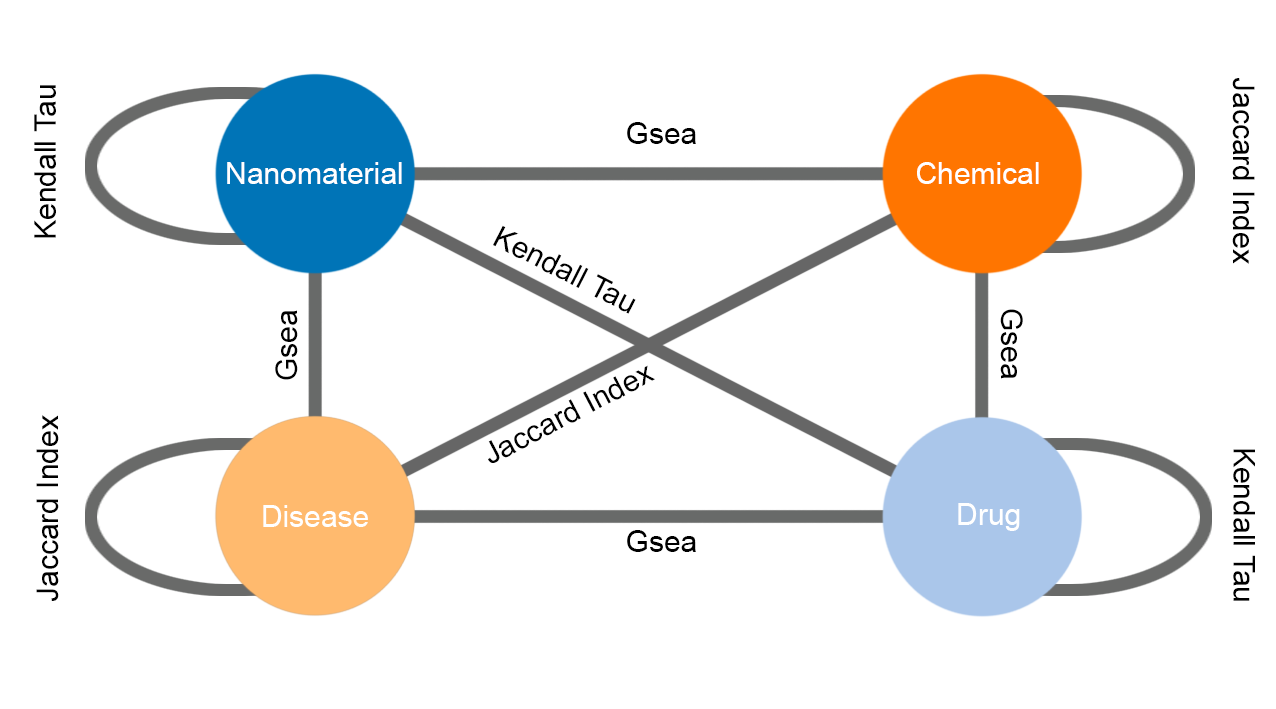
\includegraphics[scale=0.20]{img/Grafo.png}
\end{center}
E' stata calcolata la distanza per ogni coppia di entità. Tali distanze sono state poi normalizzate tra -1 e 1 per renderle confrontabili.
\end{frame}

\begin{frame}
\frametitle{Insieme di geni vs Insieme di geni}
Il Jaccard index è stato utilizzato per calcolare la similarità tra due malattie, tra due agenti chimici o tra un agente chimico e una malattia.\\
Dati due insiemi A e B \'e definito come:
\begin{equation} 
J(A, B) = \frac{|A \cap B|}{|A \cup  B|}
\end{equation}
Per ogni agente chimico vengono considerati due set di geni: quelli che sono up-regolati da quell'agente chimico e quelli che sono down-regolati.
Per quelli down-regolati il Jaccard index è calcolato con il segno negativo.
\end{frame}

\begin{frame}
\frametitle{Geni ordinati vs Geni ordinati}
La distanza Kendall Tau è stata utilizzata per calcolare la similarità tra nanomateriali e nanomateriali, tra farmaci e farmaci e tra nanomateriali e farmaci, basata sulla lista ordinata dei geni.
La distanza Kendall Tau tra due liste $T1$ e $T2$ è definita come segue:
\begin{equation}
K(T_1, T_2) = |(i, j): i < j, (T_1(i) < T_1(j) \wedge  T_2(i) > T_2(j)) \vee
\end{equation}
\begin{center}
	$ (T_1(i) > T_i(j) \wedge T_2(i) < T_2(J))  | $
\end{center}
questa distanza è compresa tra 0 e $n*(n -1)$, dove $n$ è la lunghezza della lista. 
\end{frame}

\begin{frame}
\frametitle{Geni ordinati vs insieme di geni}
La Gen Set Enrichment Analysis (GSEA), basata sul test di Kolmogorov-Smirnov, è stata usata per calcolare la similarità a coppie tra nanomateriali e malattie, tra nanomateriali e agenti chimici, tra farmaci e malattie ed infine tra farmaci e agenti chimici. Il test di KolmogorovSmirnov può essere usato per confrontare elementi con una distribuzione di probabilità. La distribuzione empirica $F_n$ per osservazioni \textit{iid}, è definito:
\begin{equation}
F_n(x) = \frac{1}{n} \sum\limits_{i=1}^n I[-\inf,x](x_i)
\end{equation}
\end{frame}

\begin{frame}
dove:
\begin{center}
$I[-\inf,x](x_i)$
\end{center}
è la funzione definita su $X$ che indica l'appartenenza di un elemento in un sottoinsieme $A$ di $X$ che ha valore 1 per tutti gli elementi di $A$ e 0 per tutti gli elementi di $X$ non in $A$. La statistica KolmogorovSmirnov per una distribuzione cumulativa $F(x)$ è 
\begin{center}
$D_n = sup_x[F_n(x)- F(x)]$
\end{center}
La statistica KolmogorovSmirnov è stata usata non in valore assoluto per preservare il segno. Ciò aiuta a capire se un gene è up o down-regolato, ovviamente anche questi valori sono stati normalizzati tra $[-1:1]$
\end{frame}

\subsection{Implementazione}
\begin{frame}
\frametitle{Implementazione}
INSIdEnano è stato implemetato usando $R$ per il back end e Javascript per il front end.
\begin{itemize}
 \item Per far comunicare i due linguaggi, sono state usate le librerie HTMLWidgets e Shiny di R. 
 \item Sistema con architettura client-server: 
 \begin{itemize}
 \item Il client è responsabile della gestione dell'interfaccia, del rendering della network, della formulazione e della sottomissione delle query. 
 \item Il server processa i dati dal database in base agli input dell'utente, e restituisce il risultato di tale computazione al client.
\end{itemize}
\end{itemize}  
\end{frame}

\section{Rendering della network}
\subsection{Problema}
\begin{frame}
\frametitle{Problema}
\begin{alertblock}{Problema}
I nodi presenti nel grafo sono 3866.
Le distanze sono state calcolate per ogni coppia di nodi del grafo. Il numero di archi è quindi pari a $3866 * 3865 \approx 15000000$.
\end{alertblock}
L'elevato numero di archi rende questo grafo:\\
\begin{center}
\textbf{INVISUALIZZABILE}
\end{center}
\end{frame}

\begin{frame}
\begin{center}
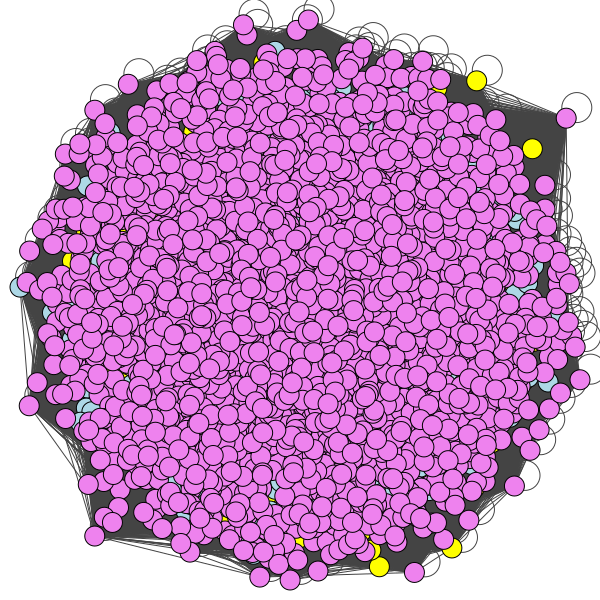
\includegraphics[scale=0.3]{img/inside.png} 
\end{center}
\end{frame}

\subsection{Soluzione}
\begin{frame}
\frametitle{Soluzione}
L'idea \'e quella di partire da un piccolo sottoinsieme di nodi, corrispondenti ai gruppi iniziali, ed organizzare l'esplorazione in maniera gerarchica. 
\begin{itemize}
\item L'utente puo' espandere una categoria alla ricerca di un particolare nodo tramite doppioclick. Tale processo \'e iterabile per ogni sottocategoria.
\item Trovato il nodo di interesse, \'e possibile visualizzare le sue connessioni con il resto del grafo cliccando sul nodo tenendo premuto alt.
\end{itemize}
\medskip
In questo modo le informazioni renderizzate sono solo quelle che l'utente ha richiesto e non tutte quelle presenti nella network. 
\end{frame}

\begin{frame}
\frametitle{Gerarchie(1/2)}
L'idea precedentemente spiegata risulta realizzabile perché sia negli agenti chimici che nei farmaci esistono delle gerarchie: Esempio:\\
\medskip
\begin{center}
''Organic Chemicals :- Dichlorophen''\\
''Enzymes and Coenzymes :- Neopterin''
\end{center}
Tale gerarchia può essere aumentata con ulteriori livelli. 
\end{frame}

\begin{frame}
\frametitle{Gerarchie (2/2)}
Nei nanomateriali e nelle malattie tali gerarchie non sono presenti.
\begin{itemize}
\item I nanomateriali possono essere visualizzati tutti in quanto sono solo 29.
\item Le malattie sono circa 600, per cui si sconsiglia di iniziare l'esplorazione da questa categoria.
\end{itemize}
\medskip
\end{frame}

\subsection{Implementazione}
\begin{frame}
\frametitle{Features}
La libreria progettata \'e stata dotata delle seguenti features:
\begin{itemize}
\item Disposizione dei nodi attraverso force layout.
\item Espansione/Compressione dei nodi categoria tramite doppioclick.
\item Messa in evidenza del vicinato di un nodo tramite shift+click.
\item Visualizzazione a richiesta delle connessioni di un nodo con tutta la network tramite alt+click.
\item Colorazione degli archi in base al valore. (verdi: positivi, rossi: negativi)
\item Spessore degli archi in base al valore.
\item Legenda in alto a sinistra per i nodi, a destra per gli archi.
\item Label su gli archi.
\item Label sui nodi.
\item Drag and drop, release.
\end{itemize}
\end{frame}

\begin{frame}
\frametitle{Implementazione}
E' stato realizzato un pacchetto R contenente una generica implementazione di un \alert{HTMLWidget}:
\begin{itemize}
	\item I file R contengono le funzioni da richiamare all'interno del codice R. Tali funzioni prendono in input i dati da renderizzare e si occupano di processarle e trasferirle alla libreria di rendering.
	\item I file javascript contengono il codice per il rendering.
\end{itemize}

Il core della nostra implementazione è la parte di rendering. Abbiamo utilizzato una libreria di visualizzazione di grafi chiamata:
\begin{center}
\href{http://d3js.org/}{d3.js}
\end{center}
\end{frame}

\begin{frame}[fragile]
\frametitle{Informazioni}
Il pacchetto creato è installabile su qualsiasi sistema operativo avente R $\geq$ 3.2.
Per installarlo e' sufficiente eseguire i seguenti comandi da terminale:
\begin{footnotesize}
\begin{lstlisting}
 $ git clone https://github.com/Abelarm/BioInf_Project.git
 $ cd BioInf_Project/graphexplorer
 $ R
 > devtools::install()
\end{lstlisting}
\end{footnotesize}
\end{frame}


\subsection{Nanocluster}

\begin{frame}
\frametitle{Nanocluster}
\begin{center}
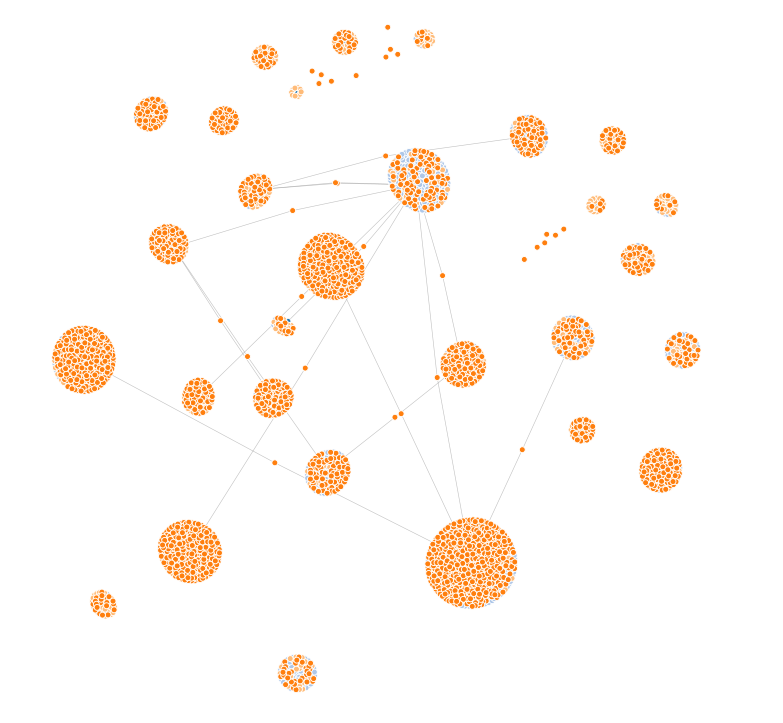
\includegraphics[scale=0.27]{img/nano_cluster_network.png} 
\end{center}
\end{frame}

\begin{frame}
\frametitle{Nanocluster}
È stato creato un'ulteriore tool per la visualizzazione di un grafo corrispondente alla network clusterizzata base ai nanomateriali.\\
\medskip
In questo caso, ogni nanomateriale \'e espandibile fino a due livelli:
\begin{itemize}
	\item Nel primo livello, vengono visualizzati nodi fittizi corrispondenti ad ogni categoria collegata al nanomateriale. 
	\item Nel secondo livello, vengono visualizzati i nodi effettivi di una certa categoria.
\end{itemize}
\end{frame}



\begin{frame}[fragile]
\frametitle{Nanocluster installation}
Per installare il tool Nanocluster e' sufficiente eseguire i seguenti comandi da terminale:
\begin{footnotesize}
\begin{lstlisting}
 $ git clone https://github.com/Abelarm/BioInf_Project.git
 $ cd BioInf_Project/nanocluster
 $ R
 > devtools::install()
\end{lstlisting}
\end{footnotesize}
\end{frame}

\section{Conclusioni}

\begin{frame}
\frametitle{Considerazioni}
\begin{itemize}
\item I pacchetti sviluppati non si prefiggono di essere strumenti a sé stanti.
\item A partire dalla visualizzazione, risulta essere più semplice verificare esistenza e forza delle connessioni.
\item Le intuizioni suggerite dalla visualizzazione grafica possono essere verificate interrogando i dati veri e propri.
\end{itemize}
\end{frame}

\begin{frame}
\frametitle{Sviluppi futuri}
\begin{itemize}
\item Rendere i tool più flessibili.
\item Produrre la documentazione relativa a quanto sviluppato per sottomettere il pacchetto al CRAN.
\end{itemize}
\end{frame}

\begin{frame}[plain]
\begin{center}
\begin{huge}
Grazie per l'attenzione.
\end{huge}
\end{center}
\end{frame}

\end{document}
